% Section content template for individual Educative lessons
% This file contains the actual content for a specific section
% Generated from Educative API section content

% Section: Evaluation of Google Maps' Design
% Section ID: 6335210467098624
% Section Slug: evaluation-of-google-maps-design
% Generated: 2025-12-07T23:06:30.276618

\subsection{Requirements compliance}\label{ygsCGbB_Y9HkygXSx2-Br}
\\
Let's see how the system we designed will handle millions of queries per second, ensuring a fast response time.

\subsubsection{Availability}\label{WZrKsEKgym5zmekiEV2Mz}
\\
With a large road network graph hosted on a single server, we ran into these issues:

\begin{itemize}
\item
\protect\phantomsection\label{ORt7SlnhzTD1MmQN2THUn}
We couldn't process user queries, since it was impossible to load such a large graph into the memory, making the system unavailable to the users.
\item
\protect\phantomsection\label{oSLE7hwPbDPY0XH_C1sjR}
It wasn't possible to make a persistent two-way connection (for navigation) between the server and millions of users per second.
\item
\protect\phantomsection\label{fRkD7TOb_inV53-lDCYfa}
It was also a single point of failure.
\end{itemize}
\\
We solved the above problems by dividing the world into small segments. Each small segment consists of a graph that can be easily loaded into a server's memory. With segments, we completed these objectives:

\begin{itemize}
\item
\protect\phantomsection\label{zrf9z-oF1J9U5DVdSfILk}
We hosted each segment on a separate server, mitigating the issue of loading a large, global graph.
\item
\protect\phantomsection\label{ztq6u-0DP0PnNUwytQenN}
The load balancer divides the request load across different segment servers depending on the user's area of search. It mitigates the issue of putting the burden on a single server, which was affecting the system's availability.
\item
\protect\phantomsection\label{8UjmEXpg5US6kFrbLtdMu}
We didn't discuss replication, but we can replicate each segment, which will help deal with a segment server as a single point of failure and distribute the request load for a segment to replicas.
\end{itemize}
\begin{quote}
\textbf{Note:} Google Maps uses lazy loading(Lazy loading is postponing the loading or initialization of resources or objects until they are needed. It reduces initial load time by reducing the amount of content to load, saves bandwidth by~delivering content to users when required, and preserves server and client resources by rendering only some of the content. Thus, it increases performance and saves system resources.) of data, putting less burden on the system, which improves availability.
\end{quote}
\\
Lazy loading reduces initial load time by reducing the amount of content to load, saves bandwidth by~delivering content to users when needed, and preserves server and client resources by rendering only some of the content.

\begin{figure}[htbp]
 \centering
 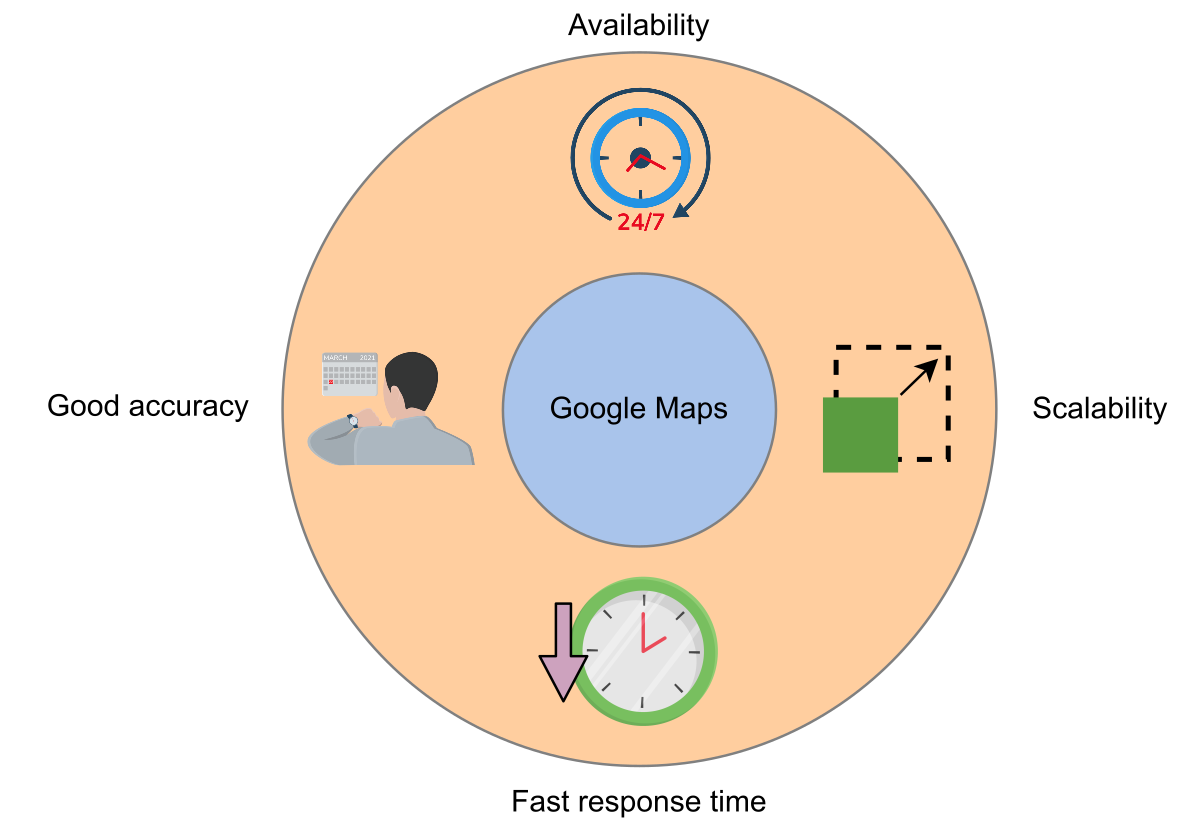
\includegraphics[width=0.25\textwidth]{Images/chapter_28/section_6335210467098624/4931788007014400.png}
 \caption{Non-functional requirements fulfilled by our maps system}
\end{figure}

\subsubsection{Scalability}\label{ERVU7WGeH2qF1b-IHqo1C}
\\
We scaled our system for large road networks. Scalability can be seen in two ways:

\begin{itemize}
\item
\protect\phantomsection\label{L2DTM2R-ZHPVTDG8uP8HQ}
The ability of the system to handle an increasing amount of user requests.
\item
\protect\phantomsection\label{3z5BTCZBbu7GjpTES1TjI}
The ability of the system to work with more data (segments).
\end{itemize}
\\
We divided the world into small segments. Each segment is hosted on a different server in the distributed system. The user requests for different routes are served from the different segment servers. In this way, we can serve millions of user requests.
\begin{quote}
\textbf{Note:} It wouldn't have been possible to serve millions of user requests if we had a single large graph spanning the whole road network. There would have been memory issues loading and processing a huge graph.
\end{quote}
\\
We can also add more segments easily because we don't have to change the complete graph. We can further improve scalability by non-uniformly selecting the size of a segment---selecting smaller segmentsizes in densely connected areas and bigger segments for the outskirts.

\subsubsection{Smaller response times}\label{bS3Cj03idaQKv7_kRwWql}
\\
We're running the user requests on small subgraphs. Processing a small subgraph of hundreds of vertices is far faster than a graph of millions of vertices. We can cache the processed small subgraph in the main memory and quickly respond to user requests. This is how our system responds to the user in less time.
\\
There's another aspect that helps our system to respond quickly, and that is keeping the segment information in the key-value store. The key-value store helps different services to get the required information quickly.

\begin{itemize}
\item
\protect\phantomsection\label{8_pw5JsnoKB4Hx6FS_m-C}
The graph processing service checks for the relevant segments in which the source and the destination latitude/longitude lie by querying the key-value store for the \texttt{segmentID} values.
\item
\protect\phantomsection\label{Zi5p7CaqhNmliQuVrwNJb}
For load-balancing user requests among different segment servers, the key-value store is queried for the \texttt{serverID} against the segment on which the graph processing should run for a specific request.
\end{itemize}

\subsubsection{Accuracy}\label{fh0Bk5yURbSL38fLs-VHv}
\\
Besides the road data we had initially, we also captured the live location data of users, on which we performed analytics using data science techniques. Our system improves the accuracy of the results (path, ETA) using these analytics. Based on the analytics of the traffic patterns, the maps are updated, and the routes and ETA estimations are improved.

\textbf{Non-functional Requirements Compliance}

\begin{table}[htbp]
\centering
\small
\adjustbox{max width=\textwidth}{
\begin{tabular}{|p{0.300\textwidth}|p{0.650\textwidth}|}
\hline
Requirements & Techniques \\
\hline
\hline
Availability & \begin{itemize} \tightlist \item Process user queries on small graphs (segments). \item Load balance requests across different segment servers. \item Replicate segment servers. \end{itemize} \\
\hline
Scalability & \begin{itemize} \tightlist \item Partition the large graphs into small graphs to ease segment addition. \item Host the segments on different servers to enable serving more queries per second. \end{itemize} \\
\hline
Less response time & \begin{itemize} \tightlist \item Cache the processed graphs. \item Use a key-value store to quickly get the required information. \end{itemize} \\
\hline
Accuracy & \begin{itemize} \tightlist \item Collect live data. \item Perform data analytics. \end{itemize} \\
\hline
\end{tabular}
}
\caption{Non-functional Requirements Compliance}
\end{table}

\subsection{Conclusion}\label{KREdKUWIuYcjc09aq7Vem}
\\
Google Maps is one of the most widely used applications in the world, where users find the shortest route between two locations. A map system models the road network with a graph data structure. To find the route, the shortest path algorithm runs over the graph. We 've seen scalability issues with a large graph of the road network. We solved the problem by splitting the world into small segments. Each segment consists of a small graph that can be loaded into the memory to find the paths quickly. We
've also seen that the estimated time of arrival can be improved by analyzing the live location data.

% End of section content